\chapter{Backtracking}
\section{Algoritmi di backtracking}

%\begin{Example}{Stringhe binarie}{}
%    \textit{Progettare un algoritmo che prende come parametro un intero $n$ e stampa tutte le stringhe binarie lunghe $n$.}
%    
%    Ad esempio per $n = 3$ l'algoritmo deve stampare $2^3 = 8$ stringhe: $000,001,010,100,011,101,110,111$.
%
%    Il meglio che ci si può augurare per un algoritmo che risolve questo problema è una complessità $\Omega(2^n*n)$.
%    \begin{lstlisting}[language=Python]
%    def bk(n, i=0, sol=[]):
%        if i==n:
%            print(''.join(sol))
%            return
%        sol.append('0')
%        bk(n,i+1,sol)
%        sol.pop()
%        sol.append('1')
%        bk(n,i+1,sol)
%        sol.pop()
%    \end{lstlisting}
%    L'albero binario di ricorsione ha $2^n-1$ nodi interni e $2^n$ foglie. Ciascun nodo interno richiede tempo $O(1)$, ciascuna foglia richiede tempo $O(n)$. La complessità dell'algoritmo è $O(2^n*n)$.
%\end{Example}

\subsection{Stringhe binarie con almeno $k$ uni}
\textit{Progettare un algoritmo che prende come parametro due interi $n$ e $k$, con $0\leq k\leq n$, e stampa tutte le stringhe binarie lunghe $n$ che contengono al più $k$ uni.}

Ad esempio: per $n=4$ e $k = 2$, delle $2^4 = 16$ stringhe lunghe $n$ bisogna stampare le seguenti 11: $0000,0001,0010,0100,1000,0011,0101,1001,0110,1010,1100$.

Un possibile algoritmo che risolve il problema in $\Theta(2^n*n)$.
\begin{lstlisting}[language=Python]
    def bk1(n, k, i=0, sol=[]):
        if i==n:
            if sol.count('1') <=k:
                print(''.join(sol))
            return
        sol.append('0')
        bk1(n, k, i+1, sol)
        sol.pop()
        sol.append('1')
        bk1(n, k, i+1, sol)
        sol.pop()
\end{lstlisting}
Indichiamo con $S(n, k)$ il numero di stringhe che bisogna stampare. Un buon algoritmo per questo problema dovrebbe avere una complessità proporzionale alle stringhe da stampare, vale a dire $O(S(n, k) * n)$ (poche stringhe = poco tempo). Ad esempio per $k = 2$ si ha
\begin{equation*}
    S(n, k) = 1 + n + \binom{n}{2} = \Theta(n ^ 2)
\end{equation*}
e quindi un buon algoritmo per $k = 2$ dovrebbe avere complessità polinomiale $O(n ^ 3)$ mentre l'algoritmo proposto ha complessità esponenziale $\Theta(2^n*n)$ (indipendente da $k$).

Osservazione: è inutile generare nell'albero di ricorsione i nodi che non hanno la possibilità di portare a soluzioni da stampare. Si ha quindi un algoritmo alternativo con un controllo sul numero di uni presenti nel prefisso delle stringhe che si vanno via via generando.
\begin{lstlisting}[language=Python]
    def bk2(n, k, i=0, tot1=0, sol=[]): 
        if i==n:
            print(''.join(sol))
            return
        sol.append('0')
        bk2(n, k, i+1, tot1, sol)
        sol.pop()
        if tot1<k:
            sol.append('1')
            bk2(n, k, i+1, tot1+1, sol)
            sol.pop()
\end{lstlisting}

Si consideri un algoritmo di enumerazione basato sul backtraking dove l’albero di ricorsione ha altezza $h$, il costo di una foglia è $g(n)$ e il costo di un nodo interno è $O(f(n))$.
Se l’algoritmo gode della seguente proprietà: un nodo viene generato solo se ha la possibilità di portare ad una foglia da stampare. Allora la complessità dell’algoritmo è proporzionale al numero di cose da stampare $S(n)$, più precisamente la complessità dell’algoritmo è:
\begin{equation*}
    O(S(n)*h*f(n) + S(n)*g(n)))    
\end{equation*}
questo perchè il costo totale dei nodi foglia sarà $O(S(n) * g(n))$ (in quanto solo le foglie
da enumerare verranno generate) e i nodi interni dell’albero che verranno effettivamente generati saranno $O(S(n) * h)$ (in quanto ogni nodo interno generato apparterrà ad un cammino che parte dalla radice e arriva ad una delle $S(n)$ foglie da enumerare).

Per l'algoritmo codificato con la funzione \verb|bk2(n, k)|, la proprietà di generare un nodo solo se questo può portare ad una delle $S(n, k)$ foglie da stampare è rispettata. Inoltre $h = n$, $g(n) = \Theta(n)$, $f(n) = O(1)$. Quindi la complessità dell'algoritmo è:
\begin{equation*}
    S(n, k) * nO(1) + S(n, k) * \Theta(n) = \Theta(S(n, k) * n)    
\end{equation*}
e l'algoritmo risulta ottimale. La complessità dell'algoritmo è $O(n ^{k + 1})$ infatti $S(n,k)= \binom{n}{0} + \binom{n}{1} + \binom{n}{2} + ... + \binom{n}{k} < 2 * n^k$.

\subsection{Stringhe binarie con esattamente $k$ uni}
\textit{Progettare un algoritmo che prende come parametro due interi $n$ e $k$, con $0\leq k\leq n$, e stampa tutte le stringhe binarie lunghe $n$ che contengono esattamente $k$ uni.}

Ad esempio: per $n=6$ e $k=3$, delle $2^6=64$ stringhe lunghe $n$ bisogna stampare le seguenti 20: $000111$, $001011$, $001101$, $001110$, $010011$, $010101$, $010110$, $011001$, $011010$, $011100$, $100011$, $100101$, $100110$, $101001$, $101010$, $101100$, $110001$, $110010$, $110100$, $111000$.

Rispetto all'esercizio precedente aggiungiamo ora una funzione di taglio anche nel caso in cui al prefisso viene aggiunto uno zero. Bisogna assicurarsi infatti che sia sempre possibile completare quel prefisso in modo da ottenere una stringa valida da stampare.

\begin{lstlisting}[language=Python]
    def bk3(n, k, i=0, tot1=0, sol=[]):
        if i==n:
            print(''.join(sol))
            return
        if tot1+n-(i+1)>=k:
            sol.append('0')
            bk3(n, k, i+1, tot1, sol)
            sol.pop()
        if tot1<k:
            sol.append('1')
            bk3(n, k, i+1, tot1+1, sol)
            sol.pop()
\end{lstlisting}
Per l'algoritmo codificato con la funzione \verb|bk3(n, k)| la proprietà di generare un nodo solo se questo può portare ad una delle $S(n, k)$ foglie da stampare è rispettata.
Inoltre, l'altezza dell'albero di ricorsione è $h = n$, il tempo richiesto da una foglia è $g(n) = \Theta(n)$ e il tempo richiesto da un nodo interno è $f(n) = O(1)$. Quindi la complessità dell'algoritmo è: 
\begin{equation*}
    S(n, k) * n*O(1) + S(n, k) * \Theta(n) = \Theta(S(n, k) * n)    
\end{equation*}
e l'algoritmo risulta ottimale.
La complessità dell'algoritmo è $O(n ^{k + 1})$ infatti $S(n, k) = \binom{n}{k}< n ^ k$.

\subsection{Stringhe sull'alfabeto}
\textit{Progettare un algoritmo che, dato un intero $n$, stampa tutte le stringhe sull’alfabeto dei 3 simboli $a$, $b$ e $c$, in cui il numero delle $b$ supera quello di ciascuno degli altri due simboli. L’algoritmo proposto deve avere complessità $O(nD(n))$ dove $D(n)$ è il numero di stringhe da stampare.}

Ad esempio per $n = 2$ l’algoritmo deve stampare la sola stringa $bb$ mentre per $n = 3$ le stringhe da stampare sono le seguenti: $bbb, abb, bab, bba, cbb, bcb, bbc$.

Per la stampa delle stringhe eseguiremo una funzione di backtracking. Al passo ricorsivo $i$-esimo possiamo potenzialmente inserire uno dei tre simboli $b$, $a$ e $c$ dell’alfabeto. Per ottenere una complessità proporzionale alle $D(n)$ stringhe da stampare la funzione di backtraking controlla che la scelta di inserire uno dei tre simboli venga fatta solo se la soluzione parziale che si ottiene porta ad un elemento da stampare. A questo proposito utilizziamo una semplice funzione di taglio che si avvale di due contatori ($na$ con il numero delle $a$ presenti nella soluzione parziale e $nc$ con il numero delle $c$ presenti nella soluzione parziale):
\begin{itemize}
    \item inseriamo il simbolo $b$ questo simbolo può sempre essere inserito;
    \item inseriamo il simbolo $a$ solo se l’inserimento di $a$ lascia spazio sufficiente per inserire eventualmente altri simboli di tipo $b$ in modo da rendere alla fine il numero di $b$ presenti nella stringa superiore a quello delle $a$ e delle $b$. Il numero delle $a$ a seguito dell’inserimento diventa $na+1$ il numero delle $b$ potenziali è $n-(na+nc+1)$ il numero delle $c$ resta $nc$. Deve quindi aversi $n-(na + nc + 1) > na +1$ e anche $n - (na + nc + 1) > nc$.
    \item inseriamo il simbolo $c$ solo se l’inserimento di $c$ lascia spazio sufficiente per inserire eventualmente altri simboli di tipo $b$ in modo da rendere alla fine il numero di $b$ presenti nella stringa superiore a quello delle $c$ e quello delle $a$. Il numero delle $c$ a seguito dell’inserimento diventa $nc + 1$ il numero delle $b$ potenziali è $n-  (na + nc + 1)$ quello delle $a$ resta $na$. Deve quindi aversi $n - (na + nc + 1) > nc +1$ e anche $n - (na + nc + 1) > na$.
\end{itemize}

\begin{lstlisting}[language=Python]
    def es(n, i=0, na=0, nc=0, sol=[]):
        if i==n:
            print(''.join(sol))
            return
        sol.append('b')
        es(n, i+1, na, nc, sol)
        sol.pop()
        if n-(na+nc+1) > na+1 and n-(na+nc+1) > nc:
            sol.append('a')
            es(n, i+1, na+1, nc, sol)
            sol.pop()
        if n-(na+nc+1) > nc+1 and n-(na+nc+1) > na:
            sol.append('c')
            es(n, i+1, na, nc+1 sol)
            sol.pop()
\end{lstlisting}
Nota che nell’albero di ricorsione prodotto dall’esecuzione di \verb|es2R| un nodo viene generato solo se porta ad una foglia da stampare. Possiamo quindi dire che la complessità dell’esecuzione di \verb|es2R(0, n, 0, 0, [ ],)| richiederà tempo:
\begin{equation*}
    O(D(n) * h * f(n) + D(n) * g(n))
\end{equation*}
dove: $h = n$ è l’altezza dell’albero, $f(n) = O(1)$ è il lavoro di un nodo interno, $g(n) = O(n)$ è il lavoro di una foglia. Quindi il costo di \verb|es2R(0, n, 0, 0, [ ],)| è $O(nD(n))$. Otteniamo quindi che il costo di \verb|es2(n)| è $O(nD(n))$.

\subsection{Sequenze valide}
Fissiamo $n$, $k$ e $T$ positivi con $T \leq nk$. Definiamo valida una sequenza di lunghezza $n$ contenente interi da 0 a $k$ e la cui somma è $T$. Ad esempio per $n = 6$, $k =4$ e $T = 12$ allora la sequenza $132042$ è valida mentre $121213$ non è valida. 

\textit{Trovate un algoritmo che dati $n$, $k$ e $T$ stampi tutte e sole le sequenze valide.  L’algoritmo deve avere complessità $O(n* k* S(n, k))$ dove $S(n, k)$ è il numero di sequenze valide esistenti.}

Utilizziamo un algoritmo di backtracking per la stampa di tutte le stringhe lunghe $n$ sull’alfabeto $\{0,...,k\}$ con l’aggiunta di una funzione di taglio. Per la funzione di taglio possiamo ragionare come segue: ad ogni inserimento nella sequenza che via via costruiamo teniamo traccia in una variabile $tot$ della somma degli interi utilizzati. Dopo l’inserimento dei primi $i-1$ valori nella sequenza, l’inserimento del valore $j$, con $0 \leq j \leq k$ avverrà se e solo se la sequenza potrà poi completarsi in modo che la somma dei suoi elementi sia almeno $T$. In altri termini l’inserimento di $j$ avviene se e solo se entrambi i seguenti vincoli sono soddisfatti: $tot + j + (n - i - 1)*k \geq T$ e $tot + j \leq T$. Grazie alla funzione di taglio la soluzione parziale via via costruita è sempre un prefisso di una soluzione da stampare.

\begin{lstlisting}[language=Python]
    def es (n, k, T, i=0, tot=0, sol=[]):
        if i==n:
            print(sol)
            return
        for j in range(k+1):
            if tot+j+(n-i-1)*k >= T and tot+j <= T:
                sol.append(j)
                es(n, k, T, i+1, tot+j, sol)
                sol.pop()
\end{lstlisting}
Nota che nell'albero di ricorsione prodotto dall'esecuzione dell'algoritmo un nodo viene generato solo se porta ad una foglia da stampare. Possiamo quindi dire che la complessità dell'esecuzione di \verb|es3(n, k, T, i=0 tot=0, sol = [])| richiederà tempo 
\begin{equation*}
    O(S(n, k) * hf(n) + S(n, k) * g(n))
\end{equation*}
dove: $h = n$ l'altezza dell'albero, $f(n) = \Theta(k)$ è il lavoro di un nodo interno, $g(n) = \Theta(n)$ è il lavoro di una foglia. Quindi il costo è $O(nkS(n, k))$.

\subsection{Stringhe di * e di caratteri crescenti}
\textit{Progettare un algoritmo che, data una stringa $X$ lunga sull'alfabeto ternario $\{0, 1, 2\}$, stampa tutte le stringhe che è possibile ottenere da $X$ sostituendo il simbolo '*' ad alcuni dei suoi caratteri in modo che i caratteri rimanenti risultino in ordine strettamente crescente. L'algoritmo proposto deve avere complessità $O(nS(X))$ dove $S(X)$ è il numero di stringhe da stampare.}

Ad esempio per $X =021$ l'algoritmo deve stampare, non necessariamente nello stesso ordine, le stringhe: $***$, $0**$, $02*$, $0*1$, $*2*$, $**1$, per $X=2110$ l'algoritmo deve stampare, non necessariamente nello stesso ordine, le stringhe: $****$, $2***$, $*1**$, $**1*$, $***0$.

Sostanzialmente nelle soluzioni che si vanno costruendo in ciascuna posizione o inseriamo il simbolo * o lasciamo il simbolo della stringa $X$. Partiamo dunque dall'algoritmo per la stampa delle stringhe binarie e aggiungiamo delle funzioni di taglio che assicurino che uno dei due simboli viene aggiunto alla soluzione parziale solo se quella soluzione potrà poi completarsi in una stringa da stampare.

Il simbolo * può sempre essere aggiunto quindi non c'è bisogno di funzione di taglio. Il simbolo della stringa può essere aggiunto solo se è il primo di questa nuova stringa o è maggiore dell'ultimo simbolo diverso da * inserito finora. C'è dunque in questo caso bisogno di una funzione di taglio.

Per far si che la funzione di taglio sia calcolabile in tempo $O(1)$ utilizziamo una variabile $p$ che tiene traccia dell'ultimo simbolo diverso da * inserito nella stringa che si va costruendo ($p = *$ se la stringa non contiene simboli diversi da *).

\begin{lstlisting}[language=Python]
    def es(X, i=0, p='*', sol=[]):
        if i==len(X):
            print(''.join(sol))
            return
        sol.append('*') 
        es(X, i+1, p, sol)
        sol.pop()
        if p=='*' or X[i] > p:
            sol.append(X[i])
            es(X, i+1, X[i] , sol)
            sol.pop()
\end{lstlisting}
Nota che nell'albero di ricorsione prodotto dall'esecuzione dell'algoritmo un nodo viene generato solo se porta ad una foglia da stampare. Possiamo quindi dire che la complessità dell'algoritmo richiederà tempo
\begin{equation*}
    O(S(X) * hf(n) + S(X) * g(n))    
\end{equation*}
dove: $h =n$ e l'altezza dell'albero, $f(n) = O(1)$ è il lavoro di un nodo interno, $g(n) = \Theta(n)$ è il lavoro di una foglia. Quindi il costo è $\Theta(n*S(X))$.

\subsection{Matrici binarie $n\times n$}
\textit{Progettare un algoritmo che prende come parametro un intero $n$ e stampa tutte le matrici binarie $n\times n$.}

Ad esempio: per $n = 2$, bisogna stampare le seguenti $2^4 = 16$ matrici:
\begin{center}
\begin{tabular}{|c|c|}\hline
     0&0\\\hline
     0&0\\\hline
\end{tabular}\hspace{0.5cm}
\begin{tabular}{|c|c|}\hline
     0&0\\\hline
     0&1\\\hline
\end{tabular}\hspace{0.5cm}
\begin{tabular}{|c|c|}\hline
     0&0\\\hline
     1&0\\\hline
\end{tabular}\hspace{0.5cm}
\begin{tabular}{|c|c|}\hline
     0&0\\\hline
     1&1\\\hline
\end{tabular}\hspace{0.5cm}
\begin{tabular}{|c|c|}\hline
     0&1\\\hline
     0&0\\\hline
\end{tabular}\hspace{0.5cm}
\begin{tabular}{|c|c|}\hline
     0&1\\\hline
     0&1\\\hline
\end{tabular}\hspace{0.5cm}
\begin{tabular}{|c|c|}\hline
     0&1\\\hline
     1&0\\\hline
\end{tabular}\hspace{0.5cm}
\begin{tabular}{|c|c|}\hline
     0&1\\\hline
     1&1\\\hline
\end{tabular}\hspace{0.5cm}\\\vspace{0.3cm}
\begin{tabular}{|c|c|}\hline
     1&0\\\hline
     0&0\\\hline
\end{tabular}\hspace{0.5cm}
\begin{tabular}{|c|c|}\hline
     1&0\\\hline
     0&1\\\hline
\end{tabular}\hspace{0.5cm}
\begin{tabular}{|c|c|}\hline
     1&0\\\hline
     1&0\\\hline
\end{tabular}\hspace{0.5cm}
\begin{tabular}{|c|c|}\hline
     1&0\\\hline
     1&1\\\hline
\end{tabular}\hspace{0.5cm}
\begin{tabular}{|c|c|}\hline
     1&1\\\hline
     0&0\\\hline
\end{tabular}\hspace{0.5cm}
\begin{tabular}{|c|c|}\hline
     1&1\\\hline
     0&1\\\hline
\end{tabular}\hspace{0.5cm}
\begin{tabular}{|c|c|}\hline
     1&1\\\hline
     1&0\\\hline
\end{tabular}\hspace{0.5cm}
\begin{tabular}{|c|c|}\hline
     1&1\\\hline
     1&1\\\hline
\end{tabular}
\end{center}

\begin{lstlisting}[language=Python]
    def es(n):
        sol = [[0]*n for _ in range(n)]
        es1(n,sol)

    def es1(n, sol, i=0 j=0):
        if i==n:
            for riga in range(n):
                print(sol[riga])
            print()
            return
        sol[i][j]=0
        if j < n-1: 
            es1(n, sol, i, j+1)
        else: 
            es1(n, sol, i+1, 0)
        sol[i][j]=1
        if j < n-1:
            es1(n, sol, i, j+1)
        else:
            es1(n, sol, i+1, 0)
\end{lstlisting}
L'albero di ricorsione è binario e di altezza $2^n$ ha dunque $2^{n^2}-1$ nodi interni e $2^{n^2}$ foglie. Ciascun nodo interno richiede tempo $O(1)$ e ciascuna foglia $O(n^2)$. L'algoritmo ha complessità $0(2^{n^2}n^2)$.

Poiché le matrici da stampare sono $2^{n^2}$ e la stampa di una matrice richiede $\Theta(n^2)$. Qualunque algoritmo per questo problema richiede tempo $\Omega(2^{n^2}n^2)$. L'algoritmo è ottimo.


\subsection{Matrici binarie $n\times n$ senza uno adiacenti}
\textit{Progettare un algoritmo che prende come parametro un intero $n$ e stampa tutte le matrici binarie $n \times n$ in cui non compaiono uni adiacenti (in orizzontale, verticale o diagonale). La complessità dell'algoritmo deve essere $O(n^2S(n))$ dove $S(n)$ è il numero di matrici da stampare.}

Ad esempio per $n=3$ delle $2^9=512$ matrici quadrate $3\times 3$ e binarie bisogna stampare le seguenti 34:
\begin{center}
\begin{tabular}{|c|c|c|}
     \hline
     0&0&0\\\hline
     0&0&0\\\hline
     0&0&0\\\hline
\end{tabular}\hspace{0.3cm}
\begin{tabular}{|c|c|c|}
     \hline
     0&0&0\\\hline
     0&0&0\\\hline
     0&0&1\\\hline
\end{tabular}\hspace{0.3cm}
\begin{tabular}{|c|c|c|}
     \hline
     0&0&0\\\hline
     0&0&0\\\hline
     0&1&0\\\hline
\end{tabular}\hspace{0.3cm}
\begin{tabular}{|c|c|c|}
     \hline
     0&0&0\\\hline
     0&0&0\\\hline
     1&0&0\\\hline
\end{tabular}\hspace{0.3cm}
\begin{tabular}{|c|c|c|}
     \hline
     0&0&0\\\hline
     0&0&0\\\hline
     1&0&1\\\hline
\end{tabular}\hspace{0.3cm}
\begin{tabular}{|c|c|c|}
     \hline
     0&0&0\\\hline
     0&0&1\\\hline
     0&0&0\\\hline
\end{tabular}\hspace{0.3cm}
\begin{tabular}{|c|c|c|}
     \hline
     0&0&0\\\hline
     0&0&1\\\hline
     1&0&0\\\hline
\end{tabular}\\\vspace{0.3cm}
\begin{tabular}{|c|c|c|}
     \hline
     0&0&0\\\hline
     0&1&0\\\hline
     0&0&0\\\hline
\end{tabular}\hspace{0.3cm}
\begin{tabular}{|c|c|c|}
     \hline
     0&0&0\\\hline
     1&0&0\\\hline
     0&0&0\\\hline
\end{tabular}\hspace{0.3cm}
\begin{tabular}{|c|c|c|}
     \hline
     0&0&0\\\hline
     1&0&0\\\hline
     0&0&1\\\hline
\end{tabular}\hspace{0.3cm}
\begin{tabular}{|c|c|c|}
     \hline
     0&0&0\\\hline
     1&0&1\\\hline
     0&0&0\\\hline
\end{tabular}\hspace{0.3cm}
\begin{tabular}{|c|c|c|}
     \hline
     0&0&1\\\hline
     0&0&0\\\hline
     0&0&0\\\hline
\end{tabular}\hspace{0.3cm}
\begin{tabular}{|c|c|c|}
     \hline
     0&0&1\\\hline
     0&0&0\\\hline
     0&0&1\\\hline
\end{tabular}\hspace{0.3cm}
\begin{tabular}{|c|c|c|}
     \hline
     0&0&1\\\hline
     0&0&0\\\hline
     0&1&0\\\hline
\end{tabular}\\\vspace{0.3cm}
\begin{tabular}{|c|c|c|}
     \hline
     0&0&1\\\hline
     0&0&0\\\hline
     1&0&0\\\hline
\end{tabular}\hspace{0.3cm}
\begin{tabular}{|c|c|c|}
     \hline
     0&0&1\\\hline
     0&0&0\\\hline
     1&0&1\\\hline
\end{tabular}\hspace{0.3cm}
\begin{tabular}{|c|c|c|}
     \hline
     0&0&1\\\hline
     1&0&0\\\hline
     0&0&0\\\hline
\end{tabular}\hspace{0.3cm}
\begin{tabular}{|c|c|c|}
     \hline
     0&0&1\\\hline
     1&0&0\\\hline
     0&0&1\\\hline
\end{tabular}\hspace{0.3cm}
\begin{tabular}{|c|c|c|}
     \hline
     0&1&0\\\hline
     0&0&0\\\hline
     0&0&0\\\hline
\end{tabular}\hspace{0.3cm}
\begin{tabular}{|c|c|c|}
     \hline
     0&1&0\\\hline
     0&0&0\\\hline
     0&1&0\\\hline
\end{tabular}\hspace{0.3cm}
\begin{tabular}{|c|c|c|}
     \hline
     0&1&0\\\hline
     0&0&0\\\hline
     1&0&0\\\hline
\end{tabular}\\\vspace{0.3cm}
\begin{tabular}{|c|c|c|}
     \hline
     0&1&0\\\hline
     0&0&0\\\hline
     1&0&1\\\hline
\end{tabular}\hspace{0.3cm}
\begin{tabular}{|c|c|c|}
     \hline
     1&0&0\\\hline
     0&0&0\\\hline
     0&0&0\\\hline
\end{tabular}\hspace{0.3cm}
\begin{tabular}{|c|c|c|}
     \hline
     1&0&0\\\hline
     0&0&0\\\hline
     0&0&1\\\hline
\end{tabular}\hspace{0.3cm}
\begin{tabular}{|c|c|c|}
     \hline
     1&0&0\\\hline
     0&0&0\\\hline
     0&1&0\\\hline
\end{tabular}\hspace{0.3cm}
\begin{tabular}{|c|c|c|}
     \hline
     1&0&0\\\hline
     0&0&0\\\hline
     1&0&0\\\hline
\end{tabular}\hspace{0.3cm}
\begin{tabular}{|c|c|c|}
     \hline
     1&0&0\\\hline
     0&0&0\\\hline
     1&0&1\\\hline
\end{tabular}\hspace{0.3cm}
\begin{tabular}{|c|c|c|}
     \hline
     1&0&0\\\hline
     0&0&1\\\hline
     0&0&0\\\hline
\end{tabular}\\\vspace{0.3cm}
\begin{tabular}{|c|c|c|}
     \hline
     1&0&0\\\hline
     0&0&1\\\hline
     1&0&0\\\hline
\end{tabular}\hspace{0.3cm}
\begin{tabular}{|c|c|c|}
     \hline
     1&0&1\\\hline
     0&0&0\\\hline
     0&0&0\\\hline
\end{tabular}\hspace{0.3cm}
\begin{tabular}{|c|c|c|}
     \hline
     1&0&1\\\hline
     0&0&0\\\hline
     0&0&1\\\hline
\end{tabular}\hspace{0.3cm}
\begin{tabular}{|c|c|c|}
     \hline
     1&0&1\\\hline
     0&0&0\\\hline
     0&1&0\\\hline
\end{tabular}\hspace{0.3cm}
\begin{tabular}{|c|c|c|}
     \hline
     1&0&1\\\hline
     0&0&0\\\hline
     1&0&0\\\hline
\end{tabular}\hspace{0.3cm}
\begin{tabular}{|c|c|c|}
     \hline
     1&0&1\\\hline
     0&0&0\\\hline
     1&0&1\\\hline
\end{tabular}
\end{center}

Per la stampa delle matrici eseguiremo una funzione di backtracking. Nella generica locazione $sol[i][j]$ è potenzialmente consentito inserire 0 o 1. Per ottenere una complessità proporzionale alle $S(n)$ matrici da stampare basta controllare che il bit inserito consenta sempre di ottenere poi una matrice da stampare. Il bit 0 può sempre essere inserito mentre per il bit 1 c’è bisogno di una funzione di taglio che controlli che nelle caselle già riempite di $sol$ adiacenti a $sol[i][j]$ non sia stato inserito un 1. Le potenziali caselle adiacenti già riempite sono le seguenti 4: $sol[i-1][j-1]$, $sol[i-1][j]$, $sol[i - 1][j + 1]$ e $sol[i][j - 1]$. Inseriamo dunque il simbolo 1 in $sol[i][j]$ solo se 
\begin{lstlisting}[language=Python]
    (i = 0 or j = 0 or sol[i-1][j-1] = 0) and
    (i = 0 or sol[i-1][j] = 0) and
    (i = 0 or j = n-1 or sol[i-1][j+1]) and
    (j = 0 or sol[i][j-1] == 0)    
\end{lstlisting}

\begin{lstlisting}[language=Python]
    def es(n):
        sol = [[0]*n for _ in range(n)]
        es1(n,sol)

    def es1(n, sol, i=0 j=0):
        if i==n:
            for riga in range(n):
                print(sol[riga])
            print()
            return
        sol[i][j] = 0
        if j < n-1:
            es1(n, sol, i, j+1)
        else: 
            es1(n, sol, i+1, 0)
        if (i==0 or j=0 or sol[i-1][j-1]==0) and \
            (i==0 or sol[i-1][j]==0) and \
            (i==0 or j==n-1 or sol [i-1][j+1]==0) and \
            (j=0 or sol[i][j-1]=0):
            sol[i][j]=1
            if j < n-1:
                es1(n, sol, i, j+1)
            else:
                es1(n, sol, i+1, 0)
\end{lstlisting}

Siano S(n) le matrici da stampare, l'algoritmo ha complessità $O(S(n) n^2)$: l'albero di ricorsione è binario e di altezza $n^2$; solo i nodi che portano ad una delle $S(n)$ soluzioni vengono effettivamente generati; i nodi interni all'albero di ricorsione effettivamente generati saranno $O(S(n) n^2)$ e le foglie effettivamente generate saranno $S(n)$; ciascun nodo interno richiede tempo $O(1)$ e ciascuna foglia richiede tempo $O(n^2)$; il tempo in totale sarà $O(S(n) n^2)+O(S(n)n^2)=O(S(n) n^2)$.

Qualunque algoritmo per questo problema richiede tempo $\Omega(S(n)n^2)$: le soluzioni da stampare sono $S(n)$ e il tempo per stampare ciascuna di queste è $\Theta(n^2)$. L'algoritmo proposto è ottimo.

\subsection{Matrici binarie $n\times n$ con righe e colonne non decrescenti}
\textit{Progettare un algoritmo che prende un intero $n$ e stampa tutte le matrici binarie di dimensioni $n\times n$ in cui righe e colonne risultano ordinate in modo non-decrescente. La complessità dell'algoritmo deve essere $O(n^2S(n))$ dove $S(n)$ è il numero di matrici da stampare.}

Ad esempio per $n = 2$ vanno stampate le seguenti 6 matrici:
\begin{center}
\begin{tabular}{|c|c|}
     \hline
     0&0\\\hline
     0&0\\\hline
\end{tabular}\hspace{0.5cm}
\begin{tabular}{|c|c|}
     \hline
     0&0\\\hline
     0&1\\\hline
\end{tabular}\hspace{0.5cm}
\begin{tabular}{|c|c|}
     \hline
     0&0\\\hline
     1&1\\\hline
\end{tabular}\hspace{0.5cm}
\begin{tabular}{|c|c|}
     \hline
     0&1\\\hline
     0&1\\\hline
\end{tabular}\hspace{0.5cm}
\begin{tabular}{|c|c|}
     \hline
     0&1\\\hline
     1&1\\\hline
\end{tabular}\hspace{0.5cm}
\begin{tabular}{|c|c|}
     \hline
     1&1\\\hline
     1&1\\\hline
\end{tabular}
\end{center}

Per la stampa delle matrici eseguiremo una funzione di backtracking. Nella generica locazione $sol[i][j]$ è potenzialmente consentito inserire 0 o 1. Per ottenere una complessità proporzionale alle $S(n)$ matrici da stampare basta controllare che il bit inserito consenta sempre di ottenere poi una matrice da stampare. Il bit 1 può sempre essere inserito mentre per il bit 0 c’è bisogno di una funzione di taglio che controlli che nelle caselle già riempite di $sol$ adiacenti a $sol[i][j]$ in orizzondate o verticale non sia stato inserito un 1. Le potenziali caselle adiacenti già riempite sono le seguenti 2: $sol[i-1][j]$ e $sol[i][j-1]$. Inseriamo dunque il simbolo 0 in $sol[i][j]$ solo se

\begin{lstlisting}[language=Python]
    (i = 0 or sol[i-1][j] = 0) and(j = 0 or sol[i][j-1] == 0)    
\end{lstlisting}

\begin{lstlisting}[language=Python]
    def es(n): 
        sol = [[0]*n for _ in range(n)]
        es1(n,sol)

    def es1(n, sol, i=0 j=0):
        if i==n:
            for riga in range(n):
                print(sol[riga])
            print() 
            return 
        if (i==0 or sol[i-1][j]==0) and (j==0 or sol[i][j-1]==0):
            sol[i][j]=0
            if j < n-1:
                es1(n, sol, i, j+1)
            else: 
                es1(n, sol, i+1, 0) 
        sol[i][j]=1 
        if j < n-1:
            es1(n, sol, i, j+1)
        else:
            es1(n, sol, i+1, 0)
\end{lstlisting}

\subsection{Permutazioni da $0$ a $n-1$}
\textit{Progettare un algoritmo che prende come parametro l'intero $n$ e stampa tutte le permutazioni dei numeri da 0 a $n-1$.}

Ad esempio per $n = 4$ bisogna stampare $4! = 24$ permutazioni: $[0,1,2,3]$ $[0,1,3,2]$ $[0,2,1,3]$ $[0,2,3,1]$ $[0,3,1,2]$ $[0,3,2,1]$ $[1,0,2,3]$ $[1,0,3,2]$ $[1,2,0,3]$ $[1,2,3,0]$ $[1,3,0,2]$ $[1,3,2,0]$ $[2,0,1,3]$ $[2,0,3,1]$ $[2,1,0,3]$ $[2,1,3,0]$ $[2,3,0,1]$ $[2,3,1,0]$ $[3,0,1,2]$ $[3,0,2,1]$ $[3,1,0,2]$ $[3,1,2,0]$ $[3,2,0,1]$ $[3,2,1,0]$.

L’albero delle permutazioni ha $\Theta(n!)$ foglie e $\Theta(n!)$ nodi interni.
\begin{equation*}
    \sum^n_{i=0}\frac{n!}{i!}\sum^\infty_{i=0}\frac{1}{i!}\sum^\infty_{i=0}\frac{2}{2^i}=n!\frac{2}{1-\frac{1}{2}}=4n!
\end{equation*}
ho usato $i!\geq\frac{2^i}{2}$ e $\sum^\infty_{i=0}x^i=\frac{1}{1-x}$ per $x<1$.

\begin{lstlisting}[language=Python]
    def es(n):
        preso = [0]*n
        es1(n, 0, [], preso)

    def es1(n, i, sol, preso):
        if i==n:
            print(sol)
            return 
        for j in range(n):
            if preso[j]==0:
                sol.append(j)
                preso[j]=1
                es1(n, i+1, sol, preso)
                sol.pop()
                preso[j]=0
\end{lstlisting}

L'algoritmo ha complessità $\Theta(n!n)$: l'albero delle permutazioni ha $\Theta(n!)$ nodi interni e $n!$ foglie $= 2^{\Theta(n\log n)}$; ciascun nodo interno richiede tempo $\Theta(n)$ e ciascuna foglia richiede tempo $\Theta(n)$.

Qualunque algoritmo per questo problema richiede tempo $\Omega(n!n)$: le soluzioni da stampare sono $n!$ e il tempo per stampare ciascuna di queste è $\Theta(n)$. L'algoritmo proposto è ottimo.

\subsection{Permutazioni da $0$ a $n-1$ con posizioni e numeri pari}
\textit{Progettare un algoritmo che prende come parametro l'intero $n$ e stampa tutte le permutazioni dei numeri da 0 a $n-1$ dove nelle posizioni pari compaiono numeri pari. La complessità dell'algoritmo deve essere $O(S(n) n^2)$ dove $S(n)$ è il numero di permutazioni da stampare.}

Ad esempio per $n = 5$ delle $5!=120$ permutazioni bisogna stampare le seguenti 12:
$[0,1,2,3,4]$ $[0,1,4,3,2]$ $[0,3,2,1,4]$ $[0,3,4,1,2]$ $[2,1,0,3,4]$ $[2,1,4,3,0]$ $[2,3,0,1,4]$$[2,3,4,1,0]$ $[4,1,0,3,2]$ $[4,1,2,3,0]$ $[4,3,0,1,2]$ $[4,3,2,1,0]$.

Per la stampa delle permutazioni eseguiremo una funzione di backtracking. Al passo ricorsivo $i$-esimo possiamo potenzialmente inserire uno degli $n$ interi non ancora inseriti. Per ottenere una complessità proporzionale alle $S(n)$ permutazioni da stampare la funzione di backtraking controlla che la scelta di inserire un intero non ancora inserito $j$ venga fatta solo se $j$ è pari e la posizione in cui inserire è pari o $j$ è dispari e la posizione in cui inserire $j$ è dispari (vale a dire $j$ modulo $2 == i$ modulo 2).

\begin{lstlisting}[language=Python]
    def es(n): 
        preso = [0]*n 
        es1(n, 0, [], preso)
    
    def es1(n, i, sol, preso):
        if i==n:
            print(sol)
            return
        for j in range(n):
            if preso[j]==0 and j%2==i%2:
                sol.append(j)
                preso[j]=1
                es1(n, i+1, sol, preso)
                sol.pop()
                preso[j]=0
\end{lstlisting}

Sia $S(n)$ il numero di permutazioni da stampare. L'algoritmo ha complessità $O(S(n)n^2)$: l'albero di ricorsione è di altezza $n$; solo i nodi che portano ad una delle $S(n)$ soluzioni vengono effettivamente generati; i nodi interni effettivamente generati saranno $O(S(n) n)$ e le foglie effettivamente generate saranno $S(n)$; ciascun nodo interno richiede tempo $\Theta(n)$ e ciascuna foglia richiede tempo $\Theta(n)$; il tempo in totale sarà $O(S(n) n)\Theta(n)+ S(n) \Theta(n)= O(S(n)n^2)$.

\subsection{Problema di ottimizzazione dello Zaino}
\textit{Abbiamo $n$ oggetti, ciascuno caratterizzato da un peso $p_i$ ed un valore $v_i$. Abbiamo inoltre uno zaino di capacità $C$. Tra tutti i possibili sottoinsiemi degli $n$ oggetti vogliamo trovare quello il cui peso non supera $C$ e il cui valore sia massimo. Il peso ed il valore di un insieme di oggetti sono dati dalla somma dei pesi e dalla somma dei valori degli oggetti dell’insieme rispettivamente. Progettare un algoritmo che prende in input la lista dei valori degli $n$ oggetti e la lista dei pesi degli $n$ oggetti e la capacità dello zaino e restituisce la soluzione al problema (la lista con gli oggetti da inserire nello zaino per massimizzarne il valore).}

Ad esempio consideriamo la seguente istanza con $C=166$ e $n= 10$ oggetti con peso e valore riportati in tabella:

\begin{center}
\begin{tabular}{|c|c|c|}
     \hline
    \textbf{oggetto}& \textbf{peso}& \textbf{valore}\\\hline
    0&23&92\\\hline
    1&31&57\\\hline
    2&29&49\\\hline
    3&89&87\\\hline
    4&44&68\\\hline
    5&53&60\\\hline
    6&38&43\\\hline
    7&63&67\\\hline
    8&85&84\\\hline
    9&82&72\\\hline
\end{tabular}
\end{center}

La soluzione ottima pesa 165, vale 309 ed il suo vettore caratteristico è $SOL=[1, 1, 1, 0, 1, 0, 1, 0, 0, 0]$.

Possiamo risolvere il problema ricorrendo ad un algoritmo esaustivo: generiamo tutti i possibili sottoinsiemi degli $n$ oggetti. Per ognuno verifichiamo se è una soluzione ammissibile (vale a dire se il peso del sottoinsieme di oggetti non eccede la capacità dello zaino) e, in questo caso, ne calcoliamo il valore. Teniamo traccia della soluzione ammissibile di valore massimo via-via trovata. Al termine diamo in outuput il massimo trovato.

Poiché i sottoinsiemi da considerare per $n$ oggetti sono $2^n$ l'algoritmo esaustivo avrà complessità esponenziale $\Omega(2^n)$.

\begin{lstlisting}[language=Python]
    def es(P, V, c):
        
        def es1(P, V, c, i, Sol):
            n=len(V)
            nonlocal Sol0, val0
            if i==n:
                if sum([P[i] for i in range(n) if Sol[i] == 1]) <= c:
                    val = sum([V[i] for i in range(n) if Sol[i]==1])
                    if val > val0:
                        Sol0 = Sol.copy(); val0 = val
            else:
                Sol.append(0)
                es1(P, V, c, i+1, Sol)
                Sol.pop()
                Sol.append(1)
                es1(P, V, c, i+1, Sol)
                Sol.pop()
    
    val0=-1; Sol0=[]
    es1(P, V, c, 0, [])
    print(val0, Sol0)
\end{lstlisting}

Non è difficile modificare il codice in modo che ogni nodo sappia il valore e il peso parziale della soluzione che si sta costruendo. In questo modo i nodi foglia possono scoprire se bisogna aggiornare la soluzione ottima in tempo $O(1)$. Nota che il numero di nodi interni da generare resta $\Theta(2^n)$ e l’asintotica dell’algoritmo risulta ora $\Theta(2^n)$. Cosa più importante, in questo modo ogni nodo interno sa quanto vale e quanto pesa la soluzione parziale costruita fino a quel momento. Queste informazioni possono risultare utili in vista dell’introduzione di eventuali funzioni di taglio.

\begin{lstlisting}[language=Python]
    def es(P, V, c):
        
        def es1(P, V, c, i, Sol, val, peso):
            n=len(V)
            nonlocal Sol0, val0
            if i==n:
                if peso <= c:
                    if val > val0:
                        Sol0 = Sol.copy(); val0 = val
            else:
                Sol.append(0)
                es1(P, V, c, i+1, Sol, val, peso)
                Sol.pop() 
                Sol.append(1)
                es1(P, V, c, i+1, Sol, val+V[i], peso+P[i])
                Sol.pop()

        val0=-1; Sol0=[]
        es1(P, V, c, 0, [], 0, 0)
        print(val0, Sol0)
\end{lstlisting}

Trasformiamo l'algoritmo di ricerca esaustiva in un algoritmo di backtraking introducendo funzioni di taglio che permetteranno di potare alcuni dei $\Theta(2^n)$ nodi presenti nell'albero di ricorsione. Nel nostro caso procederemo come segue: 
\begin{enumerate}
    \item potiamo i nodi che non portano a soluzioni ammissibili; 
    \item potiamo nodi che se anche portassero a soluzioni ammissibili queste non sarebbero tali da migliorare la soluzione ottima fino a quel momento ottenuta. 
\end{enumerate}
La funzione di taglio del punto 1 verrà applicata al figlio di destra di ogni nodo interno (dove si decide se prendere l'oggetto). La funzione di taglio del punto 2 verrà applicata al figlio di sinistra di ogni nodo interno (dove si decide di non prendere l'oggetto).

\begin{lstlisting}[language=Python]
    def es(P, V, c)
        
        def es1(P, V, c, i, Sol, val, peso):
            n=len(V)
            nonlocal Sol0, val0
            if i==n:
                if val > val0:
                    Sol0=Sol.copy(); val0=val
            else:
                Sol.append(0)
                es1(P, V, c, i+1, Sol, val, peso)
                Sol.pop()
                if peso+P[i] <= c:
                    Sol.append(1)
                    es1(P, V, c, i+1 , Sol, val+V[i], peso+P[i])
                    Sol.pop()
        
        val0=-1; Sol0=[]
        es1(P, V, c, 0, [], 0, 0)
        print(val0, Sol0)
\end{lstlisting}

Resta da implementare la seconda funzione di taglio: potare quei nodi che se anche portassero a soluzioni ammissibili queste non sarebbero tali da migliorare la soluzione ottima fino a quel momento ottenuta.

Un modo poco costoso per raggiungere parzialmente quest'obiettivo vien fuori dalla seguente semplice osservazione: se al livello $i$ della ricorsione decido di non inserire l'oggetto $i$ nello zaino, nessuna delle soluzioni ammissibili che sarà possibile ottenere potrà valere più di $val+\sum^{n-1}_{j=i+1}v_j$. Di conseguenza se $val+\sum^{n-1}_{j=i+1}v_j\leq val0$ possiamo potare l'albero di ricorsione evitando di porre $sol[i] = 0$.

L'obiettivo è raggiunto solo parzialmente perché $val+\sum^{n-1}_{j=i+1}v_j>val0$ non garantisce che le soluzioni ammissibili che sarà possibile raggiungere saranno realmente in grado di migliorare la soluzione ottima.

Per rendere efficiente il calcolo di questa funzione di taglio nel codice che segue faremo si che ogni nodo dell'albero a livello $i$ riceva, una variabile $valR$ con l'informazione del valore totale degli oggetti restanti (vale a dire $\sum^{n-1}_{j=i}v_j$).

\begin{lstlisting}[language=Python]
    def es(P, V, c):
    
        def es1(P, V, c, i, Sol, val, valR, peso):
            n=len(V)
            nonlocal Sol0, val0
            if i==n:
                if val > val0:
                    Sol0=Sol.copy(); val0=val
            else:
                if val+valR-V[i] > val0:
                    Sol.append(0)
                    es1(P, V, c, i+1, Sol, val, valR-V[i], peso)
                    Sol.pop()
                if peso+P[i] <= c:
                    Sol.append(1)
                    es1(P, V, c, i+1, Sol, val+V[i], val-RV[i], peso+P[i])
                    Sol.pop()
        val0=-1; Sol0=[]; valR=sum(V)
        es1(P, V, c, 0, [], 0, valR, 0)
        print(val0, Sol0)
\end{lstlisting}

Per il problema dello zaino quindi abbiamo visto 3 algoritmi:
\begin{itemize}
    \item \verb|Zaino(P,V,C):| algoritmo di ricerca esaustiva.
    \item \verb|Zaino1(P,V,C):| algoritmo di backtraking con una funzione di taglio.
    \item \verb|Zaino2(P,V,C):| algoritmo di backtraking con due funzioni di taglio.
\end{itemize}
L'efficacia delle funzioni di taglio per questo tipo di algoritmi può essere validata sperimentalmente.
Ad esempio possiamo introdurre nei codici dei 3 algoritmi un contatore dei nodi interni dell'albero di ricorsione effettivamente generati nel corso della loro esecuzione.

Eseguendo i tre algoritmi sull'istanza d'esempio con gli $n=10$ oggetti, vale a dire:
\begin{lstlisting}[language=Python]
    P=[23, 31, 29, 89, 44, 53, 38, 63, 85, 82]
    V=[92, 57, 49, 87, 68, 60, 43, 67, 84, 72]
    C=166
\end{lstlisting}
per i $2^n-1=1023$ nodi interni dell'albero di ricorsione si ha:
\begin{itemize}
    \item Per \verb|Zaino(P,V,C)| vengono visitati 1023 su 1023 nodi interni
    \item Per \verb|Zaino1(P,V,C)| vengono visitati 102 su 1023 nodi interni
    \item Per \verb|Zaino2(P,V,C)| vengono visitati 371 su 1023 nodi interni
\end{itemize}

In genere migliore è la funzione di taglio più questa risulta computazionalmente onerosa. Considerando che ogni nodo dell'albero di ricorsione dovrà applicarla, non sempre funzioni in grado di tagliare di più producono algoritmi più veloci.

L'effettività di alcune funzioni di taglio può dipende dalla qualità della soluzione ottima prodotta fino a quel momento. Un esempio di ciò si ha con la seconda funzione di taglio che abbiamo utilizzato per lo zaino.
In questi casi può essere fruttuoso far partire il backtraking da una soluzione di buona qualità che poi il backtraking tenterà di migliorare.
Per ottenere "buone" soluzioni da cui partire è possibile ricorrere, in una fase di preprocessing, ad algoritmi approssimanti che garantiscono di produrre soluzioni di buona qualità (anche se non ottime) in tempi contenuti.

\subsection{Problema della 3-colorazione}
\textit{Sia $G$ un grafo non diretto, una 3-colorazione di $G$ è una colorazione dei suoi nodi con 3-colori ($0, 1$ e $2$) tale che non risultino nodi adiacenti con lo stesso colore. Se una colorazione esiste possiamo rappresentarla con un vettore $sol$ dove $sol[i]$ è il colore assegnato al nodo $i$. Progettare un algoritmo che, preso un grafo $G$ restituisce una sua 3-colorazione, \texttt{None} se il grafo non è 3-colorabile.}

Possiamo risolvere il problema con un algoritmo di backtracking che va alla ricerca delle eventuali 3-colorazioni del grafo e appena ne trova una termina. Al passo ricorsivo $i$ si sceglie un colore per il nodo $i$ tra quelli non già utilizzati per $i$ nodi a lui adiacenti e se esiste si procede a colorare il nodo $i + 1$. Se si raggiunge $i=n$ l'algoritmo restituisce la colorazione.

\begin{lstlisting}[language=Python]
    def col3(G, i=0, sol=[]):
        if i==len(G):
            return sol
        C=[]
        for j in G[i]:
            if j < i and sol[j] not in C:
                C.append(sol[j])
        for c in range(3):
            if c not in C:
                sol.append(c)
                if col3(G, i+1, sol):
                    return sol    
                sol.pop()
\end{lstlisting}

La funzione di taglio introdotta (vale a dire la scelta di non colorare un vertice intermedio con un colore uguale a quello di un vertice adiacente già colorato) non garantisce che quella colorazione porterà ad una foglia che rappresenta una colorazione. La complessità quindi non sarà necessariamente proporzionale al numero di 3-colorazioni esistenti. La complessità dell’algoritmo è $O(3^n)$: l’albero di ricorsione è un albero ternario di altezza $n$ che ha dunque al più $\frac{3^n-1}{3-1}=\Theta(3^n)$ nodi (ricorda infatti che un albero $t$-ario completo, con $t > 1$, ha esattamente $\sum^n_{i=0}t^i=\frac{t^n-1}{t-1}$ nodi); ogni nodo interno richiede tempo $O(n)$ mentre al più una foglia verrà raggiunta e richiederà tempo $O(1)$. Il tempo totale è $O(3^n)$.

Dare una buona stima della complessità è piuttosto difficile proprio perché dipende fortemente dal grafo di input. Possiamo però vedere come l'algoritmo si comporta su alcuni input.

\subsection{Il problema del ciclo Hamiltoniano}
\textit{In un grafo un ciclo si dice Hamiltoniano se tocca tutti i nodi del grafo.
Dato un grafo $G$ voglimo sapere se $G$ ha o meno un ciclo Hamiltoniano. Progettare un algoritmo che preso in input il grafo $G$ restituisce un ciclo hamiltoniano se nel grafo è presente, nulla altrimenti.}

\begin{figure}[ht]
    \centering
    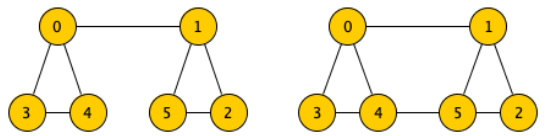
\includegraphics[width=0.6\linewidth]{images/ciclo-hamiltoniano.PNG}
    \caption{Il grafo a sinistra non ha ciclo hamiltoniano, il grafo di destra si}
    \label{fig:ciclo-hamiltoniano}
\end{figure}

Ogni nodo del grafo viene toccato una sola volta dal ciclo quindi un ciclo hamiltoniano è una permutazione $P$ degli $n$ vertici del grafo con la proprietà che esistono nel grafo tutti gli archi:
\begin{equation*}
    (P[0], P[1]), (P[1], P[2]), ..., (P[n-2], P[n-1]), (P[n-1], P[0])
\end{equation*}
per risolvere il problema possiamo quindi andare alla ricerca di una tale permutazione. Per potare lo spazio di ricerca nell'albero delle permutazioni possiamo: imporre che la permutazione inizi con il vertice 0; imporre che i prefissi della permutazione rappresentino cammini del grafo.

\begin{lstlisting}[language=Python]
    def es(G):
        presi=[0]*len(G)
        presi[0]=1
        sol=[0]
        if es1(G, 1, sol, presi):
            return sol

    def es1(G, i, sol, presi):
        if i==len(G):
            if 0 in G[sol[-1]]:
                return True
            return False
        for j in G[sol[-1]]:
            if presi[j]==0:
                sol.append(j)
                presi[j]=1
                if es1(G, i+1, sol, presi):
                    return True
                presi[j]=0
                sol.pop()
        return False    
\end{lstlisting}

La funzione di taglio introdotta (vale a dire la scelta di non generare solo permutazioni che cominciano con 0 e i cui prefissi siano cammini del grafo) non garantisce che i nodi generati porteranno ad una foglia che rappresenta un ciclo hamiltoniano. La complessità quindi non sarà necessariamente proporzionale al numero di cicli hamiltoniani esistenti.
La complessità dell’algoritmo è $O(n!)$: l’albero di ricorsione è un albero delle permutazioni di altezza $n-1$ che ha dunque al $O((n-1)!)$; ogni nodo interno richiede tempo $\Theta(n)$ mentre al più $(n-1)!$ foglie verranno raggiunte e ciascuna richiederà tempo $O(1)$. Il tempo totale è $O((n-1)! n) = O(n!)$.

La complessità del programma dipende fortemente dal grafo di input. Ci sono grafi per i quali trova subito un ciclo Hamiltoniano (ad es. se il grafo è un ciclo) o determina che non ce ne sono (ad es. se il grafo è un albero). Ma ci sono tantissimi grafi per i quali impiega tempo esponenziale per dare una risposta. Basti pensare che se il grafo G non ha cicli Hamiltoniani, tutti i cammini dal nodo 1 saranno comunque visitati e se questi sono tanti la complessità sarà molto elevata.

\subsection{Il problema delle $n$ regine}
\textit{Data una scacchiera $n\times n$ vogliamo calcolare quanti diversi modi ci sono di disporre sulla scacchiera $n$ regine in modo che nessuna di esse sia in grado di catturarne un'altra in base alle regole degli scacchi. Perciò una disposizione dovrà prevedere che nessuna delle $n$ regine abbia colonna, riga o diagonale in comune con un altra.}

Ad esempio, ecco due delle possibile disposizioni per $n = 8$:
\begin{center}
\begin{tabular}{|c|c|c|c|c|c|c|c|}
    \hline
     &&&&&&&$x$\\\hline
     &$x$&&&&&&\\\hline
     &&&$x$&&&&\\\hline
     $x$&&&&&&&\\\hline
     &&&&&&$x$&\\\hline
     &&&&$x$&&&\\\hline
     &&$x$&&&&&\\\hline
     &&&&&$x$&&\\\hline
\end{tabular}\hspace{0.5cm}
\begin{tabular}{|c|c|c|c|c|c|c|c|}
    \hline
     &&&$x$&&&&\\\hline
     &$x$&&&&&&\\\hline
     &&&&&&$x$&\\\hline
     &&$x$&&&&&\\\hline
     &&&&&$x$&&\\\hline
     &&&&&&&$x$\\\hline
     $x$&&&&&&&\\\hline
     &&&&$x$&&&\\\hline
\end{tabular}
\end{center}

Bisogna quindi progettare una funzione di backtracking che prende come parametro l’intero $n$ e restituisce il numero di disposizioni lecite possibili. Non è difficile convincersi che per $n = 2$ ed $n = 3$ non esiste alcuna disposizione lecita. Per i primi valori di $n$ la funzione deve dare le seguenti risposte:
\begin{center}
\begin{tabular}{|c|r|}
     \hline
    \textbf{n}&\textbf{disposizioni}\\\hline
    1&1\\\hline
    2&0\\\hline
    3&0\\\hline
    4&2\\\hline
    5&10\\\hline
    6&4\\\hline
    7&40\\\hline
    8&92\\\hline
    9&352\\\hline
    10&724\\\hline
    11&2680\\\hline
    12&14200\\\hline
    13&73712\\\hline
    14&365596\\\hline
    15&2279184\\\hline
\end{tabular}
\end{center}

Le disposizioni che vogliamo contare soddisfano 3 vincoli:
\begin{enumerate}
    \item le $n$ regine sono su righe distinte;
    \item le $n$ regine sono su colonne distinte;
    \item le $n$ regine sono su diagonali distinte.
\end{enumerate}
I primi due vincoli fanno si che in ciascuna delle disposizioni da contare in ogni riga della scacchiera ci sarà esattamente una regina e lo stesso varrà per ogni colonna. Questo significa che posso vedere ciascuna delle disposizioni da contare come una permutazione dei numeri da 0 a $n-1$ dove in posizione $i$ compare la colonna in cui è stata sistemata la regina della $i$-esima riga.
\begin{center}
\begin{tabular}{|c|c|c|c|c|c|c|c|}
    \hline
     &&&&&&&$x$\\\hline
     &$x$&&&&&&\\\hline
     &&&$x$&&&&\\\hline
     $x$&&&&&&&\\\hline
     &&&&&&$x$&\\\hline
     &&&&$x$&&&\\\hline
     &&$x$&&&&&\\\hline
     &&&&&$x$&&\\\hline
\end{tabular}\hspace{0.5cm}
\begin{tabular}{|c|}
    \hline
     7\\\hline
     1\\\hline
     3\\\hline
     0\\\hline
     6\\\hline
     4\\\hline
     2\\\hline
     5\\\hline
\end{tabular} $=[7, 1, 3, 0, 6, 4, 2, 5]$
\end{center}

Una disposizione che soddisfa i primi due vincoli del problema (vale a dire regine in righe e colonne distinte) può dunque essere vista come una permutazione dei primi $n$ interi. Non tutte le permutazioni corrispondono alle disposizioni lecite che vogliamo contare. Esempio di permutazione che non corrisponde ad una disposizione lecita per il problema delle $n$ regine (la regina sulla riga 2 e quella sulla riga 5 condividono la stessa diagonale)
\begin{center}$[7, 1, 3, 0, 4, 6, 2, 5]=$ 
\begin{tabular}{|c|}
    \hline
     7\\\hline
     1\\\hline
     3\\\hline
     0\\\hline
     4\\\hline
     6\\\hline
     2\\\hline
     5\\\hline
\end{tabular}
\begin{tabular}{|c|c|c|c|c|c|c|c|}
    \hline
     &&&&&&&$x$\\\hline
     &$x$&&&&&&\\\hline
     &&&\textcolor{red}{$x$}&&&&\\\hline
     $x$&&&&&&&\\\hline
     &&&&$x$&&&\\\hline
     &&&&&&\textcolor{red}{$x$}&\\\hline
     &&$x$&&&&&\\\hline
     &&&&&$x$&&\\\hline
\end{tabular}\hspace{0.5cm}
\end{center}

Per risolvere il problema possiamo modificare il programma che stampa tutte le permutazioni dei primi $n$ interi in modo che, anziché stamparle, conti quelle che soddisfano i vincoli richiesti.

Cominciamo a scrivere il programma per il conteggio delle "soluzioni" che soddisfanno solo i primi due vincoli quando si richiede alle regine di non essere mai nelle stesse righe o stesse colonne (in pratica conta le permutazioni lunghe $n$ restituendo $n!$), aggiungeremo poi a questa versione del programma delle funzioni di taglio in modo che vengano generate (e quindi contate) solo permutazioni corrispondenti a disposizioni lecite.
\begin{lstlisting}[language=Python]
    def es(n):
        presi=[0]*n
        return es1(n, 0, [], presi)

    def es1(n, i, sol, presi): 
        if i==n:
            return 1
        tot = 0
        for j in range(n): 
            if presi[j]==0:
                sol.append(j)
                presi[j]=1
                tot += es1(n, i+1, sol, presi)
                sol.pop()
                presi[j]=0
        return tot
\end{lstlisting}

Bisogna ora aggiungere al codice i vincoli attinenti alle diagonali di modo che la posizione che si vuole assegnare ad una nuova regina non deve essere su una diagonale già occupata. Ogni cella della scacchiera appartiene a due diagonali: una diagonale che va da sinistra a destra (diagonale principale DP) ed una diagonale che va da destra a sinistra (diagonale secondaria DS). Ecco due proprietà che permettono di ricavare da una cella la diagonale a cui questa appartiene. 

Due celle $(i, j)$ e $(i', j')$ sono sulla stessa diagonale principale DP se e solo se $i - j = i' - j'$, due celle $(i, j)$ e $(i', j')$ sono sulla stessa diagonale secondaria DS se e solo se $i + j = i' + j'$.

In un insieme DP posso tener traccia delle diagonali già occupate che vanno da sinistra a destra mentre in un insieme DS posso tener traccia delle diagonali già occupate che vanno da destra a sinistra. Per sapere se la diagonale DP della cella $(i,j)$ è stata già occupata basta vedere se $i-j$ è in DP, analogamente, per sapere se la diagonale DS della cella $(i,j)$ è stata già occupata basta vedere se $i+j$ è in DS.
\begin{lstlisting}[language=Python]
    def es(n):  
        presi=[0]*n 
        return es1(n, 0, [], presi, set(), set())

    def es1(n, i, sol, presi, DP, DS):
        if i==n:
            return 1
        tot = 0
        for j in range(n):
            if presi[j]==0 and (i-j not in DP) and (i+j) not in DS):
                sol.append(j)
                presi[j]=1; DP.add(i-j); DS.add(i+j)
                tot += es1(n, i+1, sol, presi, DP, DS)
                sol.pop()
                presi[j]=0; DP.remove(i-j); DS.remove(i+j)
        return tot
\end{lstlisting}
